\documentclass[conference]{IEEEtran}

%XXX Remove before final submission
\usepackage{todonotes}
\usepackage{cite}
\usepackage{amsmath}
\usepackage{caption}
\usepackage{subcaption}
% Note that the amsmath package sets \interdisplaylinepenalty to 10000
% thus preventing page breaks from occurring within multiline equations. Use:
%\interdisplaylinepenalty=2500
% after loading amsmath to restore such page breaks as IEEEtran.cls normally
\usepackage{url}
\usepackage{hyperref}
\usepackage{verbatim}
\usepackage{siunitx}
\usepackage{listings}

\lstdefinelanguage{Julia}{
  basicstyle=\small\ttfamily,
  showspaces=false,
  showstringspaces=false,
  keywordstyle={\textbf},
  morekeywords={if,else,elseif,while,for,begin,end,quote,try,catch,return,local,abstract,function,stagedfunction,macro,ccall,finally,typealias,break,continue,type,global,module,using,import,export,const,let,bitstype,do,in,baremodule,importall,immutable},
  escapeinside={~}{~},
  morecomment=[l]{\#},
%  commentstyle=\textsf,
  commentstyle={},
  morestring=[b]",
}

\lstset{language=Julia,basicstyle=\footnotesize\ttfamily,breaklines=true}

% correct bad hyphenation here
\hyphenation{}


\begin{document}

%XXX remove before submission
\newcommand{\TODO}[1]{\todo[inline]{#1}}
\newcommand{\TODOFIG}[1]{\missingfigure{#1}}

\title{Which Program Is Slower? Hypothesis Testing for Performance Regressions}

% author names and affiliations
% use a multiple column layout for up to three different
% affiliations
\author{\IEEEauthorblockN{Jiahao Chen and Jarrett Revels}
\IEEEauthorblockA{Computer Science and Artificial Intelligence Laboratory\\
Massachusetts Institute of Technology\\
Cambridge, Massachusetts 02139--4307\\
Email: \{jiahao,jrevels\}@csail.mit.edu}
}

% make the title area
\maketitle

%%%%%%%%%%%%%%%%%%%%%%%%%%%%%%%%%%%%%%%%%%%%%%%%%%%%%%%%%%%%%%%%%%%%%%%%%%%%%%%%%%%%%%%%%%%%
\begin{abstract}
We propose a rigorous methodology for automated microbenchmarking and regression detection
in the presence of timer error, OS jitter and other environmental fluctuations. By examining
data obtained from Julia microbenchmarks, we demonstrate the ways in which timing
distributions can violate many of the statistical assumptions made by other benchmarking
frameworks. From our experimental observations, we construct a model and an accompanying
microbenchmarking strategy which purposefully avoids these assumptions. This strategy makes
efficient use of user time constraints by simultaneously maximizing the number of
measurements per trial while minimizing inter-measurement timing variations, rendering it
suitable for continuous integration (CI) pipelines, even when applied to relatively large
benchmark suites. Using our model, we formulate a robust, nonparametric hypothesis test that
makes use of the bootstrap resampling method to estimate the statistical significance of
observed variations in execution time. We test our methodology on a small collection of mock
Julia benchmarks, discussing where it succeeds relative to other methods as well as pointing
out potential pitfalls. Finally, we discuss a prototype implementation of the proposed
method that was recently released to aid in the development of the Julia language and
ecosystem, which has already caught and prevented several performance regressions in Julia's
base library.
\end{abstract}

\IEEEpeerreviewmaketitle

\TODO{come up with better section/subsection names}

%%%%%%%%%%%%%%%%%%%%%%%%%%%%%%%%%%%%%%%%%%%%%%%%%%%%%%%%%%%%%%%%%%%%%%%%%%%%%%%%%%%%%%%%%%%%
\label{sec:intro}
\section{Introduction}

Developers of high performance applications often rely on microbenchmark suites to determine
the impact of code changes on program performance. Despite the importance of these suites in
safeguarding against performance regressions, developers often run and interpret them in an
ad hoc manner. The disregard for proper interpretation wastes development time and may
lead to misguided development decisions that worsen performance.

In this paper, we consider the problem of developing a microbenchmark suite
suitable for a continuous integration (CI) workflow. We define a microbenchmark
as a benchmark whose expected execution time is on the order of 1 microsecond
or shorter,
The goal is to detect reproducibly and automatically when performance regressions occurred,
while running the entire suite in a reasonable amount of time.
In practice, the complexity of modern hardware and software enviroments introduce
undesirable variations across timing measurements of the same benchmark, which
reduce the reliability of detecting performance regressions.
Furthermore, a single execution of a microbenchmark is too short to measure
accurately by a system timer. Thus, it is necessary to execute the
microbenchmarks multiple times to obtain an accurate timing measurement.

\paragraph{The effects of timer noise}
\TODO{Cite strategies for orchestrating performance counters}

\paragraph{Controlling for environmental effects}
Modern hardware and operating systems introduce many confounding factors that
complicate a developer's ability to reason about variations in user-space
application performance~\cite{HP5e}.

At the hardware level, changes in temperature, workload, and power availability
can trigger CPU clock frequency scaling to limit power consumption.

At the operating system level, sources of variation are often referred to as
OS jitter.
Jitter may be caused by randomizing security features like address space layout
randomization (ASLR)~\cite{Shacham2004},
virtual memory management~\cite{Oyama2014,Oyama2016},
or even suboptimal process- and thread-level scheduling~\cite{Lozi2016}.
Even seemingly irrelevant configuration parameters like the size of the
OS environment can confound reproducibility. Changing the size of the
environment moves the call stack, which is loaded after the environment, which
in turn changes the alignment of data in memory~\cite{Mytkowicz2009}.

The choice of programming language compiler parameters can result in yet
further timing variations.
For compiled languages, the linker is free to choose the binary layout of the
library or executable arbitrarily, resulting in nondeterministic memory
layouts~\cite{Georges2008}.
Additionally, the behavior of the runtime can change depending on OS or hardware
parameters. For example, changing the heap size can affect garbage collector
performance~\cite{Blackburn2004}.

Most of these studies focus on Java programming language and/or the Linux OS.
While the phenomena described clearly apply to general software and hardware environments,
mitigating strategies are often highly specialized, ranging from custom OS
\cite{Akkan2012}\TODO{Cite NIX, Tessellation}, custom compilers providing
reproducible~\cite{Georges2008} or consistently randomized~\cite{Curtsinger2013}
binary layouts, to low-variability garbage collectors~\cite{Huang2004}.
These mechanisms for achieving quiescence are platform dependent, deviate strongly
from a typical user's machine and configuration, or cannot be reasonably automated without
root access to the user's machine. Reliance on these techniques could negatively impact
portability and thus decrease the likelihood of adoption.

\subsection{Designing an experimental protocol is hard}

\TODO{cite/discuss Kalibera's paper on ``benchmarking in reasonable time'', and similar
papers}

\subsection{Doing stastistics on timing measurements is hard}
\begin{figure}
\centering
\begin{subfigure}{0.22\textwidth}
    \centering
    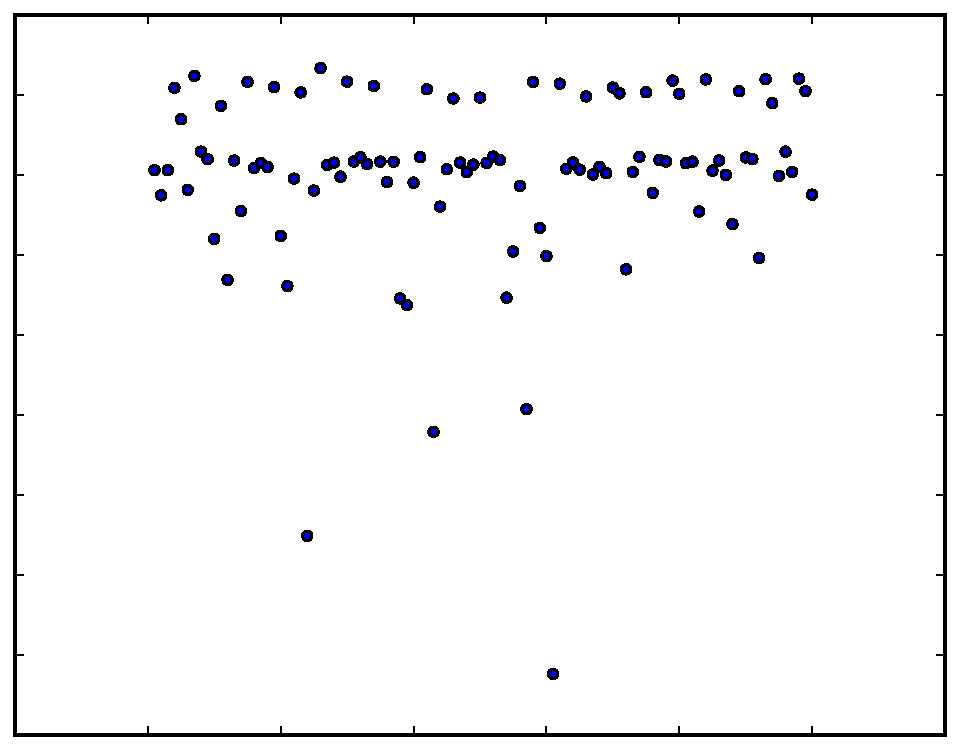
\includegraphics[width=\textwidth]{figures/fig1/simple_branchsum_fast}
    \caption{Benchmark 1: Unimodal}
\end{subfigure}%
~
\begin{subfigure}{0.22\textwidth}
    \centering
    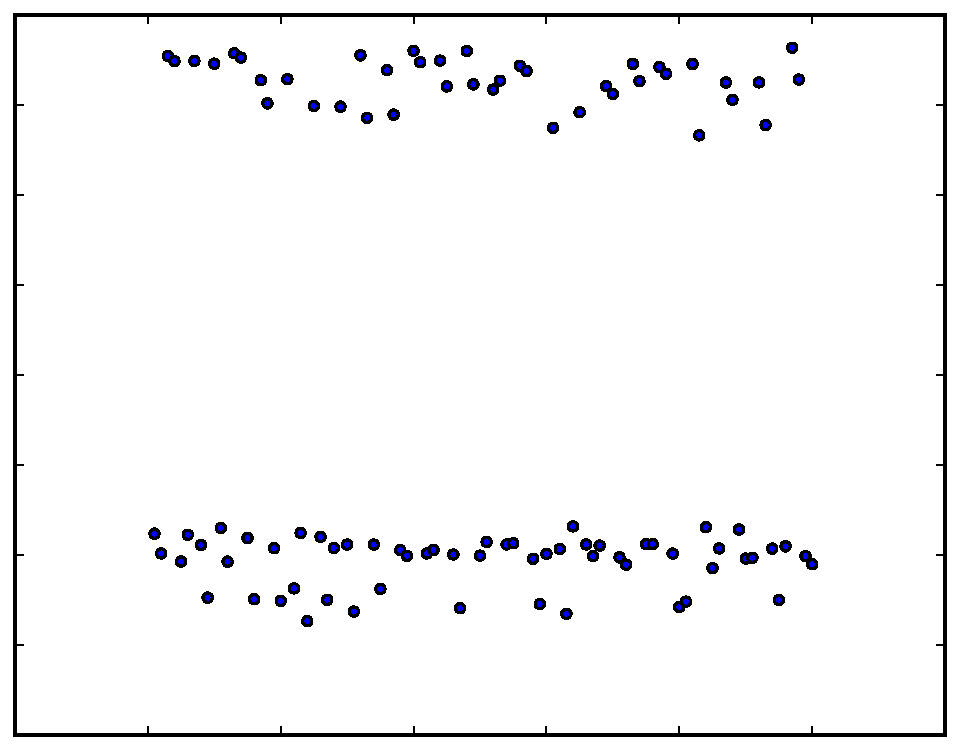
\includegraphics[width=\textwidth]{figures/fig1/bimodal_branchsum}
    \caption{Benchmark 2: Bimodal}
\end{subfigure}
\begin{subfigure}{0.22\textwidth}
    \centering
    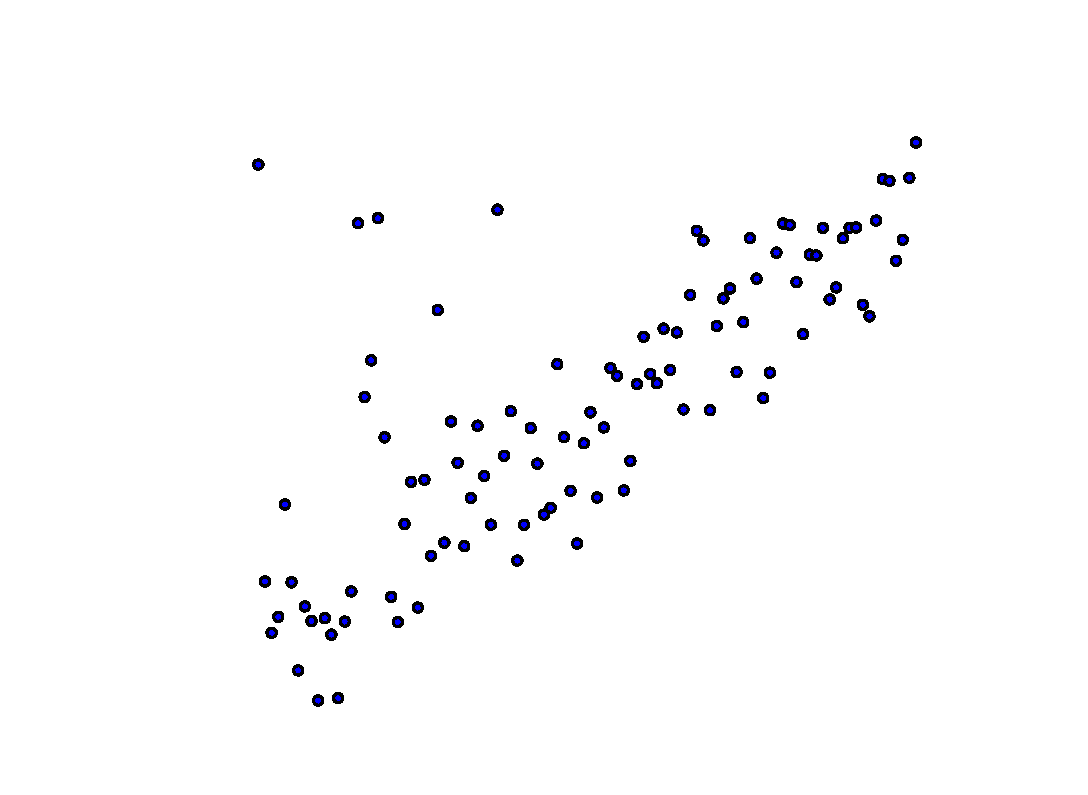
\includegraphics[width=\textwidth]{figures/fig1/drift_manyallocs_slow}
    \caption{Benchmark 3: Skewed}
\end{subfigure}
~
\begin{subfigure}{0.22\textwidth}
    \centering
    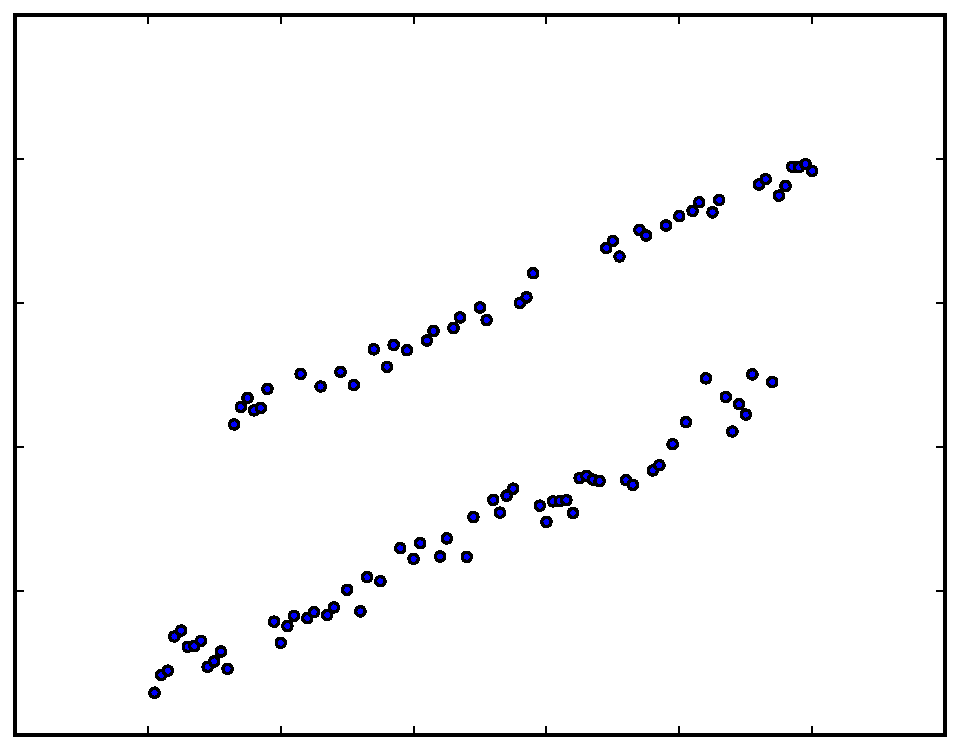
\includegraphics[width=\textwidth]{figures/fig1/bimodal_drift_sumindex}
    \caption{Benchmark 4: Bimodal + Skewed}
\end{subfigure}
\caption{Mean distributions for 4 different benchmarks. Each point is the mean time for a
         trial of 10,000 measurements. The x-axis is the index of the trial, while the
         y-axis is time.}
\label{fig:meandistributions}
\end{figure}

\TODO{cite/discuss papers that assume normality and/or that all benchmark timings are
identically distributed}

%%%%%%%%%%%%%%%%%%%%%%%%%%%%%%%%%%%%%%%%%%%%%%%%%%%%%%%%%%%%%%%%%%%%%%%%%%%%%%%%%%%%%%%%%%%%
\label{sec:notation}
\section{Notation}

The rest of this paper utilizes a consistent notation for discussing the various statistical
and measured quantities related to microbenchmarking. We define this notation here:

\begin{itemize}
    \item
    $P_0$, $P$ and $Q$ denote \textbf{benchmarkable programs}, each defined by a tape of
    instructions.

    \item
    $I^{[i]}_{P}$ is the $i^{\textrm{th}}$ \textbf{instruction} in the tape defining program $P$.
    Instruction indices are always written using bracketed superscripts, $\cdot^{[i]}$.

    \item
    $D^{[i]}_{P}$ is the \textbf{delay instruction} associated with $I^{[i]}_{P}$. Delay
    instructions are precisely defined in Section~\ref{sec:model}.

    \item
    $T_i$ is a \textbf{timing measurement}. Specifically, $T_i$ is the amount of time taken
    to perform $n_i$ \textbf{executions} of a benchmarkable program. This quantity is
    directly measurable via experiment.

    \item
    $t$ is an \textbf{execution time}. Specifically, $t$ is the amount of time it takes to
    perform a single execution of a benchmarkable program. This quantity is not generally
    measured directly but is instead derived as $t_i = T_i / n_i$.

    \item
    \textbf{Estimated quantities} are denoted with a hat, $\hat\cdot$. For example,
    $\hat{t}_{\textrm{min}}$ is the estimated value for the minimum value of the benchmark execution
    time.

    \item
    \textbf{Resampled quantities} are denoted with a superscript asterisk, $\cdot^*$. For
    example, $t^*_1, \dots t^*_m$ is a resample of $t_1, \dots t_n$.

    \item
    A benchmark \textbf{experiment} is a recipe for obtaining multiple timing measurements
    for a benchmarkable program. Experiments can be executed to obtain \textbf{trials}. The
    $i^{\textrm{th}}$ trial of an experiment is a collection of timing measurements
    $T^{\{i\}}_1, \dots T^{\{i\}}_j, \dots T^{\{i\}}_k$. Trial indices are always
    written using embraced superscripts, $\cdot^{\{i\}}$.

    \item
    $\tau$ denotes time quantities that are external to the benchmarkable program:
    \begin{itemize}
        \item $\tau_{\textrm{budget}}$ is the \textbf{time budget} for an experiment.
        \item $\tau_{\textrm{acc}}$ is the \textbf{accuracy} of the system timer.
        \item $\tau_{\textrm{prec}}$ is the \textbf{precision} of the system timer.
    \end{itemize}

    \item
    $\epsilon^{(i)[j]} = x^{(i)[j]} \tau^{(i)}$ is the \textbf{time delay} due to the
    $i^{\textrm{th}}$ \textbf{delay factor} for delay instruction $D^{[j]}$.  Specifically,
    $\tau^{(i)}$ is the factor's \textbf{time scale} and $x^{(i)[j]}$ is the factor's
    \textbf{trigger coefficient} for $D^{[j]}$. Delay factor indices are written using
    parenthesized superscripts, $\cdot^{(i)}$.

    \item
    $E_P^{(i)}$ is the total \textbf{cumulative delay} due to the $i^{\textrm{th}}$ delay
    factor during the execution of program $P$.

    \item
    $X^{(i)}_P$ is the total \textbf{cumulative trigger count} of the $i^{\textrm{th}}$
    delay factor during the execution of program $P$.

    \item
    $\nu(t)$ is an \textbf{oracle function} that, given an execution time $t_P$, estimates
    an appropriate $n_P$ necessary to overcome measurement error due to insufficient
    $\tau_{\textrm{acc}}$ and $\tau_{\textrm{prec}}$.

    \item
    $f_X(\xi)$ is the \textbf{probability density function (pdf)} associated with the random
    variable $X$. $\int_{x}^{x+\delta x} f_X(\xi) d\xi$ is the probability that $x < X <
    x+\delta x$.
\end{itemize}

%%%%%%%%%%%%%%%%%%%%%%%%%%%%%%%%%%%%%%%%%%%%%%%%%%%%%%%%%%%%%%%%%%%%%%%%%%%%%%%%%%%%%%%%%%%%
\label{sec:model}
\section{A better statistical interpretation of microbenchmark timing distributions}

In this section, we present a statistical description of microbenchmark behavior that avoids
problematic assumptions of normality or identical timing distributions between benchmarks.
This model will drive the design of our experimental protocol and hypothesis testing
formulation, discussed in future sections.

\subsection{The underlying model for program execution}

Consider an initial benchmarkable user program $P_0$, whose output is deterministic and
identical for every execution. $P_0$ can be specified by as a sequence of instructions
$I^{[i]}$:

\begin{equation}
    P_0 = \left[I^{[1]}, I^{[2]}, \dots I^{[k]}\right]
\end{equation}

We define an \textit{instruction} as a specification of a state transition that takes the
executing machine from an initial state to a desired output state. In an idealized universe,
we could assume that the state transition for instruction $I^{[i]}$ takes exactly
$\tau^{[i]}$ time, such that the total runtime of $P_0$ is $t_{P_0} = \sum_{i=1}^N
\tau^{[i]}$.

In reality, the machine and operating system within which $P_0$ runs are vulnerable to the
factors described in Section~\ref{sec:challenges}. These factors may cause the computer to
undergo zero or more intermediary state transitions before achieving the state transistion
specified by instruction $I^{[i]}$. Since these factors \textit{delay} the completion of the
original instructions, we refer to them as \textit{delay factors}\footnote{Technically,
there are some causes of timing variations which might speed up the execution of a program,
such as frequent scaling \TODO{cite}. However, these factors number far fewer than those
that slow down execution of a program, and as such, are more easily controlled. Thus, we
only focus on the latter, which we have seen to stochastically dominate the former
\TODO{Jiahao: fix this abuse of terminology}}. We can account for these delay factors by
modeling them as ``delay instructions'' $D^{[i]}$, which are interleaved with $P_0$'s
original instructions to produce a new program $P$:

\begin{equation}
    P = \left[I^{[1]}, D^{[1]}, I^{[2]}, D^{[2]}, \dots I^{[k]}, D^{[k]}\right]
\end{equation}

While the semantics of $P_0$ and $P$ are identical, the presence of the delay instructions
means that $t_P \ge t_{P_0}$, since $t_P = t_{P_0} + \sum_{j} \tau_{D^{[j]}}$, where
$\tau_{D^{[j]}}$ is the execution time of $D^{[j]}$.

$\tau_{D^{[j]}}$ can be further decomposed into the runtime contributions of individiual
delay factors. Let us imagine the delay factor $i$ can discretely ``trigger'' once during
the execution of $D^{[j]}$ with probability $p^{(i)}$.Assuming that every triggering of $i$
takes a fixed time $\tau^{(i)}$, we can express $D^{[j]}$'s runtime as the \textit{random
variable} $\tau_{D^{[j]}} = \sum_{i=1} x^{(i)}_j \tau^{(i)}$, where $x^{(i)}_j$ is a boolean
\textit{trigger coefficient}. Summing the trigger coefficients for the $i^{\textrm{th}}$
delay factor over all delay instructions gives us a \textit{trigger count}
$X_P^{(i)}$ for the entire program $P$.

Our final expression for $t_P$ in terms of these quantities is:

\begin{align}
t_P &= t_{P_0} + \sum_{j} \tau_{D^{[j]}} = t_{P_0} + \sum_{i} X_P^{(i)} \tau^{(i)} \\
    &= t_{P_0} + \sum_{j} \sum_{i} x^{(i)[j]} \tau^{(i)}
\end{align}

\TODO{Should we still discuss the various distributions that can arise from the limiting behaviors of the model?}

Note that if $\sum_{i} X_P^{(i)} = 0$, then $t_P = t_{P_0}$. For some machines, this ideal
behavior may not be possible, but there must be at least one trigger count configuration
which minimizes $t_P$ to some value $[t_P]_{\textrm{min}}$, invoking the fewest possible
delay factors that lead to smallest possible increase in execution time over $t_{P_0}$.
Rephrasing this property in the language of statisitics, there must exist some critical time
$[t_P]_{\textrm{min}}$ for which the probability density function (pdf) $f_{t_P}(\xi)$ of
$t_P$ obeys $f_{t_P}(\xi) = 0 \; \forall \; \xi < [t_P]_{\textrm{min}}$

\subsection{The model for timing measurements}

Before our model is complete, we must account for measurement error due to \textit{timer
accuracy}.

%%%%%%%%%%%%%%%%%%%%%%%%%%%%%%%%%%%%%%%%%%%%%%%%%%%%%%%%%%%%%%%%%%%%%%%%%%%%%%%%%%%%%%%%%%%%
\label{sec:protocol}
\section{Experimental protocol for benchmark execution}

\begin{figure}
\centering
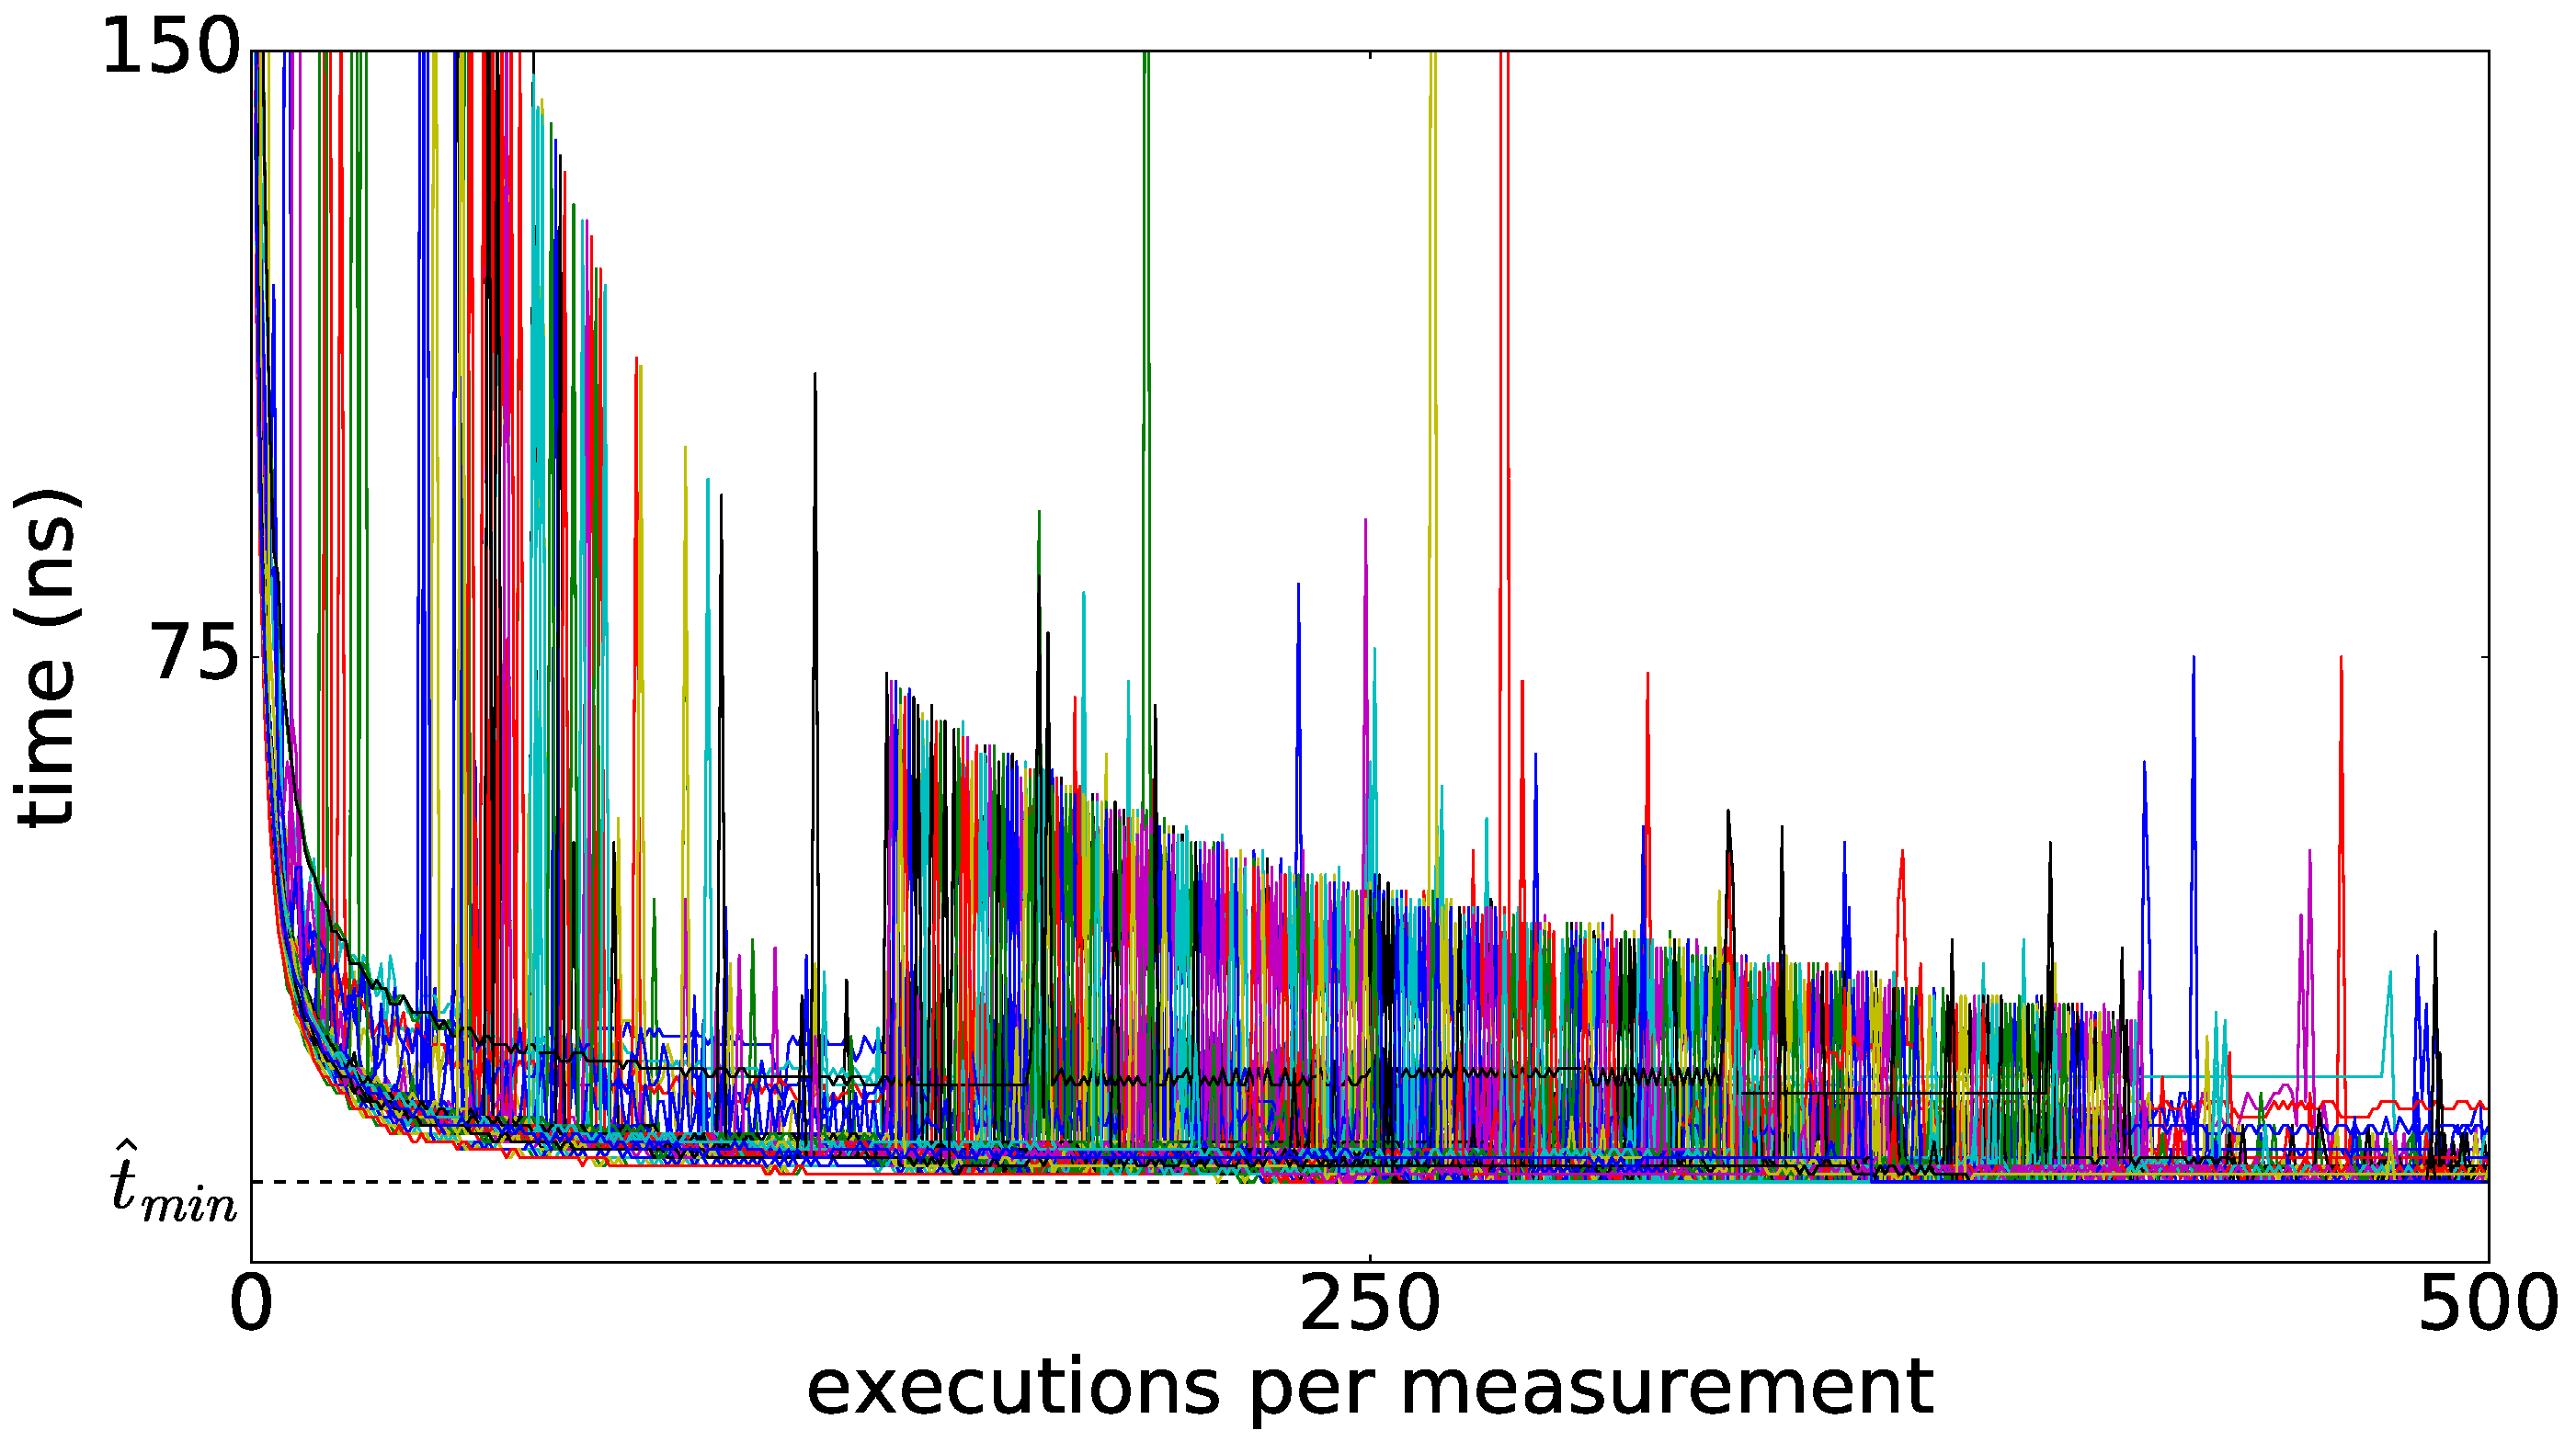
\includegraphics[width=0.45\textwidth]{figures/fig2/linear_scan_branchsum}
\caption{A plot of many trials for a single benchmark, where each trial scans through
increasing values for $n$. Note the smooth curve and asymptotic lower bound of the minima
$(n^{(i)}, [\hat{t}_{\textrm{min}}]^{(i)}_n)$.}
\label{fig:scaling}
\end{figure}

Given a benchmarkable program $P$ and a time budget $\tau_{budget}$, we'd like to define
$n$, the number of executions of $P$ to perform for each timing measurement, such that a
trial of our experiment...

\begin{itemize}
    \item ...produces timing estimates as close to the lower bound $t_{min}$ as possible
    \item ...minimizes the variance between timing measurements
    \item ...maximizes the number of timing measurements we are able to obtain under the
    constraint of $\tau_{budget}$
\end{itemize}

Given a timer accuracy $\tau_{acc}$ and a timer precision $\tau_{prec}$, our algorithm for
tuning $n$ is as follows:

\begin{enumerate}
    \item For $n \in \{1...\tau_{acc}\}$, measure the amount of time it takes to perform $n$
    executions of $P$. The result of this step is a collection of timing measurements $T_n$
    for all $n$.
    \item From the derived timing estimates $t_i = T_i / i$, select the minimum timing
    estimate $\hat{t}_{min}$.
    \item To obtain $n$, plug $\hat{t}_{min}$ into an oracle function $\nu(t_i) \to n_i$.
    Given $\tau_{acc}$ and $\tau_{prec}$, the properties of $\nu(t)$ are as follows:
    \begin{itemize}
        \item $\nu(\tau_{prec}) \approx \tau_{acc}$
        \item $\nu(\tau_{acc}) \approx \text{small} (\sim 10)$
        \item $\nu(t \gg \tau_{acc}) \approx 1$
        \item $\frac{d\nu}{dt}\big|_{t \approx \tau_{prec}} = \text{close to zero}$
        \item free of discontinuities \TODO{how to say this correctly since the range is
        discretized}
    \end{itemize}
\end{enumerate}

%%%%%%%%%%%%%%%%%%%%%%%%%%%%%%%%%%%%%%%%%%%%%%%%%%%%%%%%%%%%%%%%%%%%%%%%%%%%%%%%%%%%%%%%%%%%
\label{sec:hypotesting}
\section{Hypothesis tests for regression detection}

\begin{figure}
\centering
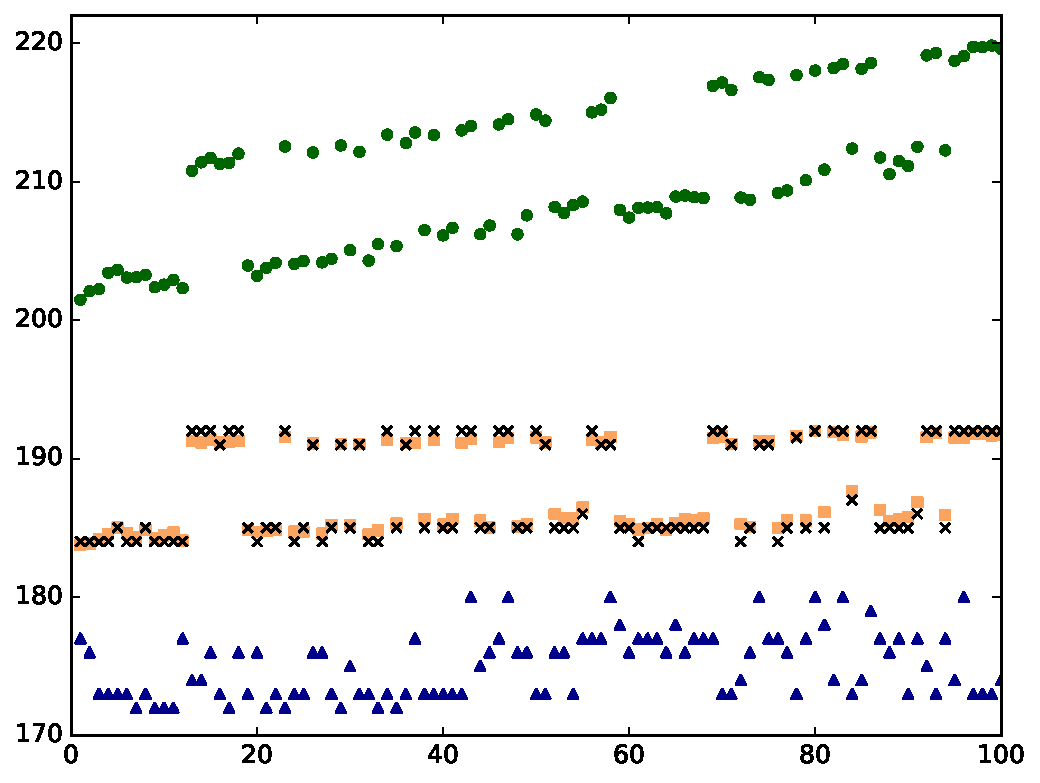
\includegraphics[width=\columnwidth]{figures/fig3/location_estimators_sumindex}
\caption{The behavior of different location parameters across multiple trials of
the \lstinline|sumindex| benchmark: mean (green filled circles), trimmed mean of
the 5th---95th percentiles (brown filled squares), medisn (black crosses), and
minimum (blue filled triangles).}
\label{fig:locationmeasures}
\end{figure}

%%%%%%%%%%%%%%%%%%%%%%%%%%%%%%%%%%%%%%%%%%%%%%%%%%%%%%%%%%%%%%%%%%%%%%%%%%%%%%%%%%%%%%%%%%%%
\label{sec:limits}
\section{Limitations of our methodology}

\begin{figure}[!t]
\centering
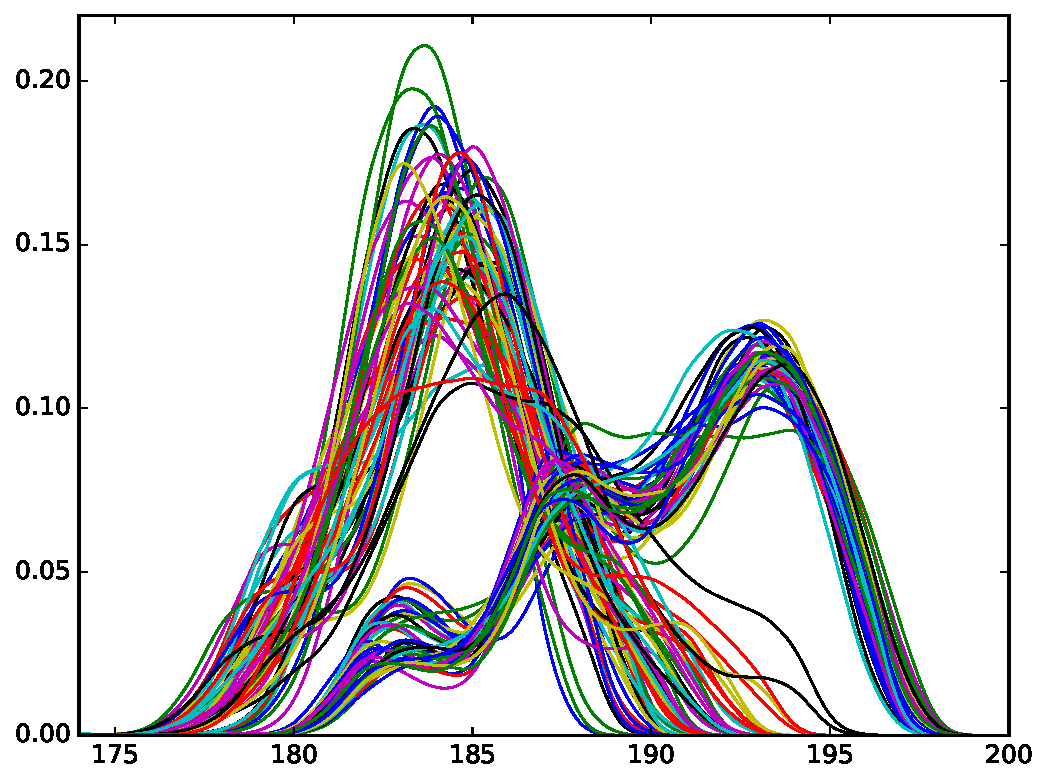
\includegraphics[width=\columnwidth]{figures/fig4/kde_pdf_sumindex}
\caption{Probability density functions (pdfs) from repeated trials of the
\lstinline|sumindex| benchmark. The pdfs form two distinct clusters, indicating
correlation across multiple trials.}
\label{fig:pdfsumindex}
\end{figure}

%%%%%%%%%%%%%%%%%%%%%%%%%%%%%%%%%%%%%%%%%%%%%%%%%%%%%%%%%%%%%%%%%%%%%%%%%%%%%%%%%%%%%%%%%%%%
\label{sec:julia}
\section{Implementation in Julia}

%%%%%%%%%%%%%%%%%%%%%%%%%%%%%%%%%%%%%%%%%%%%%%%%%%%%%%%%%%%%%%%%%%%%%%%%%%%%%%%%%%%%%%%%%%%%
\label{sec:conclusion}
\section{Conclusion}

%%%%%%%%%%%%%%%%%%%%%%%%%%%%%%%%%%%%%%%%%%%%%%%%%%%%%%%%%%%%%%%%%%%%%%%%%%%%%%%%%%%%%%%%%%%%
\label{sec:acknowledgement}
\section*{Acknowledgment}

We thank the many Julia developers, in particular Andreas Noack for many insightful
discussions. This work was supported by the Nanosoldier grant.\TODO{Get grant info}

%%%%%%%%%%%%%%%%%%%%%%%%%%%%%%%%%%%%%%%%%%%%%%%%%%%%%%%%%%%%%%%%%%%%%%%%%%%%%%%%%%%%%%%%%%%%
\bibliography{biblio}
\bibliographystyle{IEEEtran}

% that's all folks
\end{document}
\grid
